\documentclass{ximera}
%\usepackage{todonotes}

\usepackage{tkz-euclide}
\usetikzlibrary{backgrounds} %% for boxes around graphs
\usetikzlibrary{shapes,positioning}  %% Clouds and stars
\usetkzobj{all}
\usepackage[makeroom]{cancel} %% for strike outs
%\usepackage{mathtools} %% for pretty underbrace % Breaks Ximera
\usepackage{multicol}


\newcommand{\RR}{\mathbb R}
\renewcommand{\d}{\,d}
\newcommand{\dd}[2][]{\frac{d #1}{d #2}}
\renewcommand{\l}{\ell}
\newcommand{\ddx}{\frac{d}{dx}}
\newcommand{\zeroOverZero}{$\boldsymbol{\tfrac{0}{0}}$}
\newcommand{\numOverZero}{$\boldsymbol{\tfrac{\#}{0}}$}
\newcommand{\dfn}{\textbf}
\newcommand{\eval}[1]{\bigg[ #1 \bigg]}
\renewcommand{\epsilon}{\varepsilon}
\renewcommand{\iff}{\Leftrightarrow}

\DeclareMathOperator{\arccot}{arccot}
\DeclareMathOperator{\arcsec}{arcsec}
\DeclareMathOperator{\arccsc}{arccsc}


\colorlet{textColor}{black} 
\colorlet{background}{white}
\colorlet{penColor}{blue!50!black} % Color of a curve in a plot
\colorlet{penColor2}{red!50!black}% Color of a curve in a plot
\colorlet{penColor3}{red!50!blue} % Color of a curve in a plot
\colorlet{penColor4}{green!50!black} % Color of a curve in a plot
\colorlet{penColor5}{orange!80!black} % Color of a curve in a plot
                                      \colorlet{fill1}{blue!50!black!20} % Color of fill in a plot
\colorlet{fill2}{blue!10} % Color of fill in a plot
\colorlet{fillp}{fill1} % Color of positive area
\colorlet{filln}{red!50!black!20} % Color of negative area
\colorlet{gridColor}{gray!50} % Color of grid in a plot

\pgfmathdeclarefunction{gauss}{2}{% gives gaussian
  \pgfmathparse{1/(#2*sqrt(2*pi))*exp(-((x-#1)^2)/(2*#2^2))}%
}



\newcommand{\fullwidth}{}
\newcommand{\normalwidth}{}



%% makes a snazzy t-chart for evaluating functions
\newenvironment{tchart}{\rowcolors{2}{}{background!90!textColor}\array}{\endarray}

%%This is to help with formatting on future title pages.
\newenvironment{sectionOutcomes}{}{} 

\author{Emma Smith Zbarsky}
\license{Creative Commons Attribution 3.0 Unported}
\acknowledgement{https://quadbase.org/questions/q14499v1}
\begin{document}

\begin{exercise}

Consider the intersection of two country roads shown below. If a cow is
ambling away from the intersection at a leisurely 3 miles per hour and a
cowherd is running toward the intersection at a blazing 10 miles per
hour, what is the speed at which the cowherd is approaching the cow when
he is 2 miles away from the intersection and the cow passed the
intersection 40 minutes earlier?



\begin{image}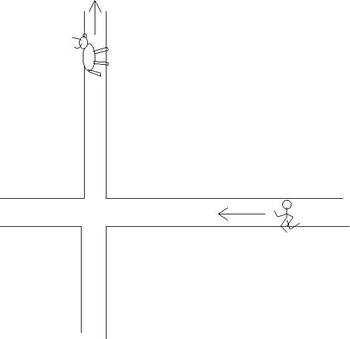
\includegraphics{relatedrates-cow.jpg}\end{image}


\begin{hint}
This is a related rates problem. You need to begin by identifying your
variables, finding a relation, differentiating the relation and plugging
in known (and/or computed) values to find the desired rate.
\end{hint}


\begin{hint}
\begin{image}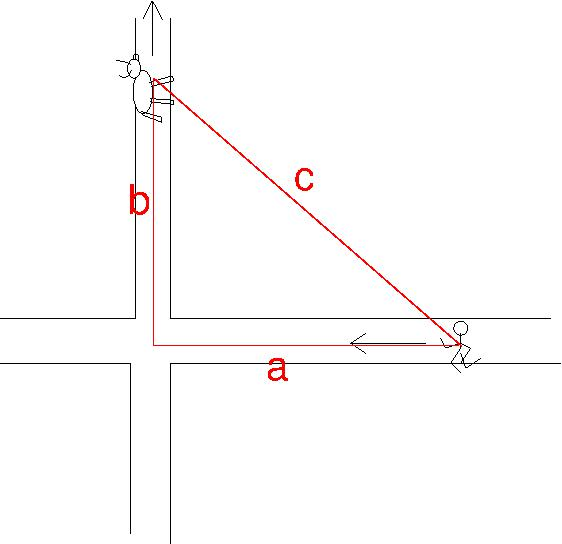
\includegraphics{rr-cow-labeled.jpg}\end{image}



Variables

\begin{itemize}
\item
  $a$ is the distance from the cowherd to the intersection in miles
\item
  $b$ is the distance from the cow to the intersection in miles
\item
  $c$ is the distance from the cow to the cowherd in miles
\end{itemize}

Relation

\begin{itemize}
\itemsep1pt\parskip0pt\parsep0pt
\item
  $a^2+b^2 = c^2$
\end{itemize}

Known values

\begin{itemize}
\item
  $a = 2$ miles
\item
  $b = 3$ miles/hour $*2/3$ hours = 2 miles
\item
  $c = \sqrt{2^2+2^2} = \sqrt{8}$ miles
\item
  $\frac{da}{dt} = -10$ miles per hour
\item
  $\frac{db}{dt} = 3$ miles per hour
\end{itemize}

Want to know?

\begin{itemize}
\itemsep1pt\parskip0pt\parsep0pt
\item
  $\frac{dc}{dt}$
\end{itemize}

Differentiate

\begin{itemize}
\itemsep1pt\parskip0pt\parsep0pt
\item
  $2a\frac{da}{dt} + 2b\frac{db}{dt} = 2c\frac{dc}{dt}$
\end{itemize}

Plugging in: \begin{align*}
2(2)\left(-10\right) + 2(2)\left(3\right) &= 2(\sqrt{8})\frac{dc}{dt} \\
\frac{dc}{dt} &= \frac{-40+12}{2\sqrt{8}} \\
&= -\frac{14}{\sqrt{8}} \\
&= -\frac{7}{\sqrt{2}}
\end{align*} So the cowherd is closing on the cow at a rate of
$\frac{7}{\sqrt{2}} \simeq 4.95$ miles per hour.
\end{hint}


\begin{multipleChoice}
\choice{The cowherd is approaching the cow at $0$ miles per hour.}
\choice[correct]{The cowherd is approaching the cow at $\frac{7}{\sqrt{2}}$ miles per
hour.}
\choice{The cowherd is approaching the cow at $\frac{7}{2}$ miles per hour.}
\choice{The cowherd is approaching the cow at $\frac{13}{\sqrt{2}}$ miles per
hour.}
\choice{The cowherd is approaching the cow at $\frac{11}{\sqrt{8}}$ miles per
hour.}
\end{multipleChoice}

\end{exercise}
\end{document}
